\documentclass[mathserif, 10pt]{beamer}
\usepackage[utf8]{inputenc}
\usepackage{amsmath, amsfonts}
\usepackage{appendixnumberbeamer}
\usepackage{verbatim}

\newcommand{\ACPmix}{\ensuremath{A_{CP}^{\rm{mix}}}}

\title[A Glance into Flavour Physics...]{A Glance into Flavour Physics \\with Effective Field Theories\\ and Machine Learning}
\author[Jorge Alda]{Jorge Alda,\\ Universidad de Zaragoza/CAPA\\
Università degli Studi di Padova/INFN \hspace{2em} \texttt{jalda@unizar.es} }

\date[PhD Thesis]{28th April 2022}



\usetheme{Zaragoza}
\usecolortheme{Unizar}
\titlepagelogoA{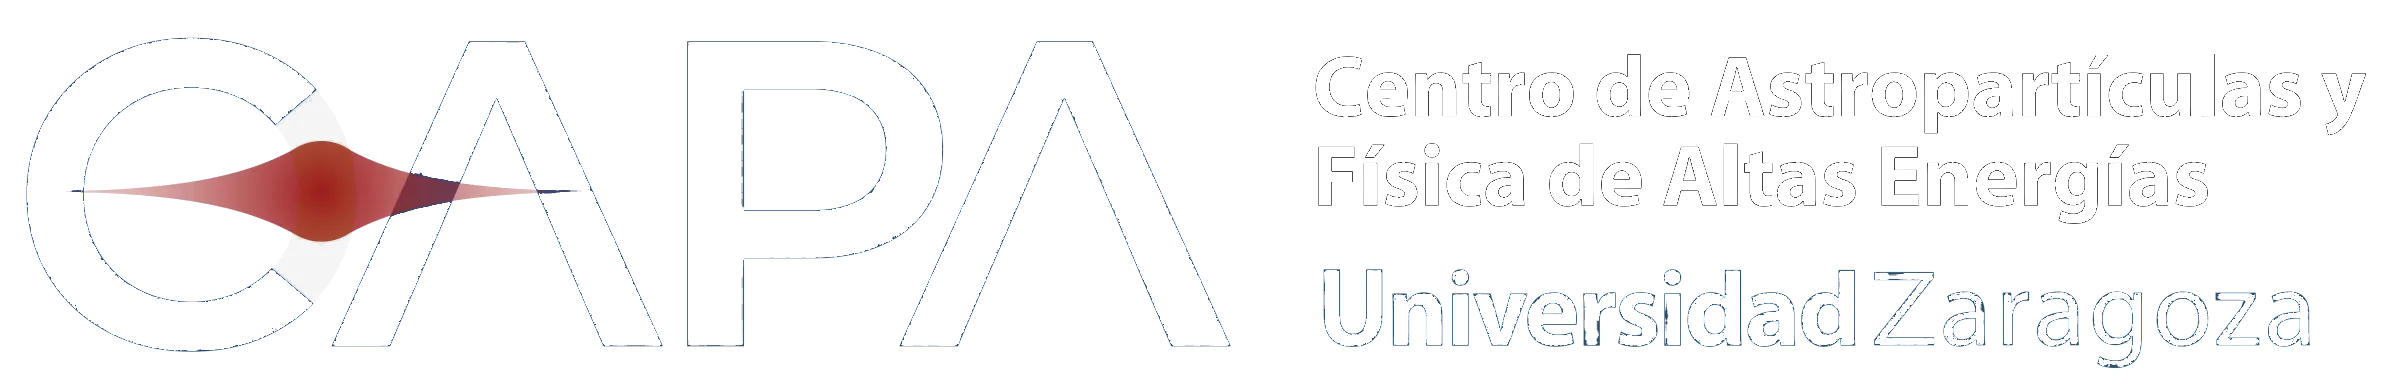
\includegraphics[width=6cm]{logos/CAPA.png}}
\titlepagelogoB{
\includegraphics[width=4cm]{logos/dftuz2.png}}


\newcommand\colorcite[1]{{\scriptsize\color{blue}#1}}

\begin{document}
\begin{frame}[noframenumbering,plain]

\titlepage

\end{frame}

\begin{frame}\frametitle{Publication List}

    \begin{itemize}
        \item J. Alda, J. Guasch, S. Peñaranda,
              \textit{Some Results on Lepton Flavour Universality Violations,}\\
              Eur. Phys. J. C 79.7 (2019), p.588, arXiv:1805.03636 [hep-ph].
        \item J. Alda, J. Guasch, S. Peñaranda, \textit{Anomalies in B meson decays: A phenomenological approach,}\\
              Eur. Phys. J. Plus 137 (2022), p.217, arXiv: 2012.14799 [hep-ph].
        \item J. Alda, J. Guasch, S. Peñaranda,
              \textit{Using Machine Learning techniques in phenomenological studies in flavour physics,}\\
              arXiv:2109.07405 [hep-ph].
        \item J. Alda, A. W. M. Guerrera, S. Peñaranda, S. Rigolin,
              \textit{Leptonic Meson Decays into invisible ALP,}\\
              arXiv:2111.02536 [hep-ph].
    \end{itemize}

\end{frame}

\begin{frame}\frametitle{Part I: $B$ physics}
\end{frame}

\begin{frame}\frametitle{$B$ anomalies}

    Flavour-changing neutral currents $b \to s \ell^+ \ell^-$, with $\ell = e, \mu$.
    \begin{itemize}
        \item Universality ratios $R_{K^{(*)}}$
              $$R_{K^{(*)}} = \frac{\mathrm{BR}(B\to K^{(*)}\mu^+ \mu^-)}{\mathrm{BR}(B\to K^{(*)}e^+ e^-)}\,, $$
              In the SM, theoretically clean, and $R_{K^{(*)}}=1$.\\
              LHCb measurements\footnote{R. Aaij \textit{et al.} (LHCb) arXiv:2103.11769, arXiv:1705.05802}:
              \begin{itemize}
                  \item $R_{K^+} = 0.846^{+0.042}_{-0.039}{}^{+0.013}_{-0.012}$,
                  \item $R_{K^{*0}} = 0.685^{+0.113}_{-0.069}\pm0.047$. ($3.1\,\sigma$ tension)
              \end{itemize}
        \item Angular observables for $B\to K^* \ell^+\ell^-$: $P'_4$, $P'_5\ldots$
        \item Also $B_s \to \phi \mu^+ \mu^-$ decays.
    \end{itemize}

\end{frame}

\begin{frame}\frametitle{$B$ anomalies}
    Flavour-changing charged currents $b\to c \ell \nu$, with $\ell = e/\mu, \tau$.
    \begin{columns}
        \begin{column}{0.55\textwidth}

            \begin{itemize}
                \item Universality ratios $R_{D^{(*)}}$
                      $$R_{D^{(*)}} = \frac{\mathrm{BR}(B\to D^{(*)}\tau \nu)}{\mathrm{BR}(B\to D^{(*)}\ell \nu)}\,, $$
                      $$R_D = 0.340 \pm 0.027 \pm 0.013\,,$$
                      $$R_{D^*} = 0.295 \pm 0.011 \pm 0.008\,.$$
Combined tension of $3.08\,\sigma$.\footnotemark[2]
                \item Longitudinal polarization of $D^*$.
                \item Also $B_c \to J/\psi \ell\nu$ decays.
            \end{itemize}

        \end{column}
        \begin{column}{0.5\textwidth}
            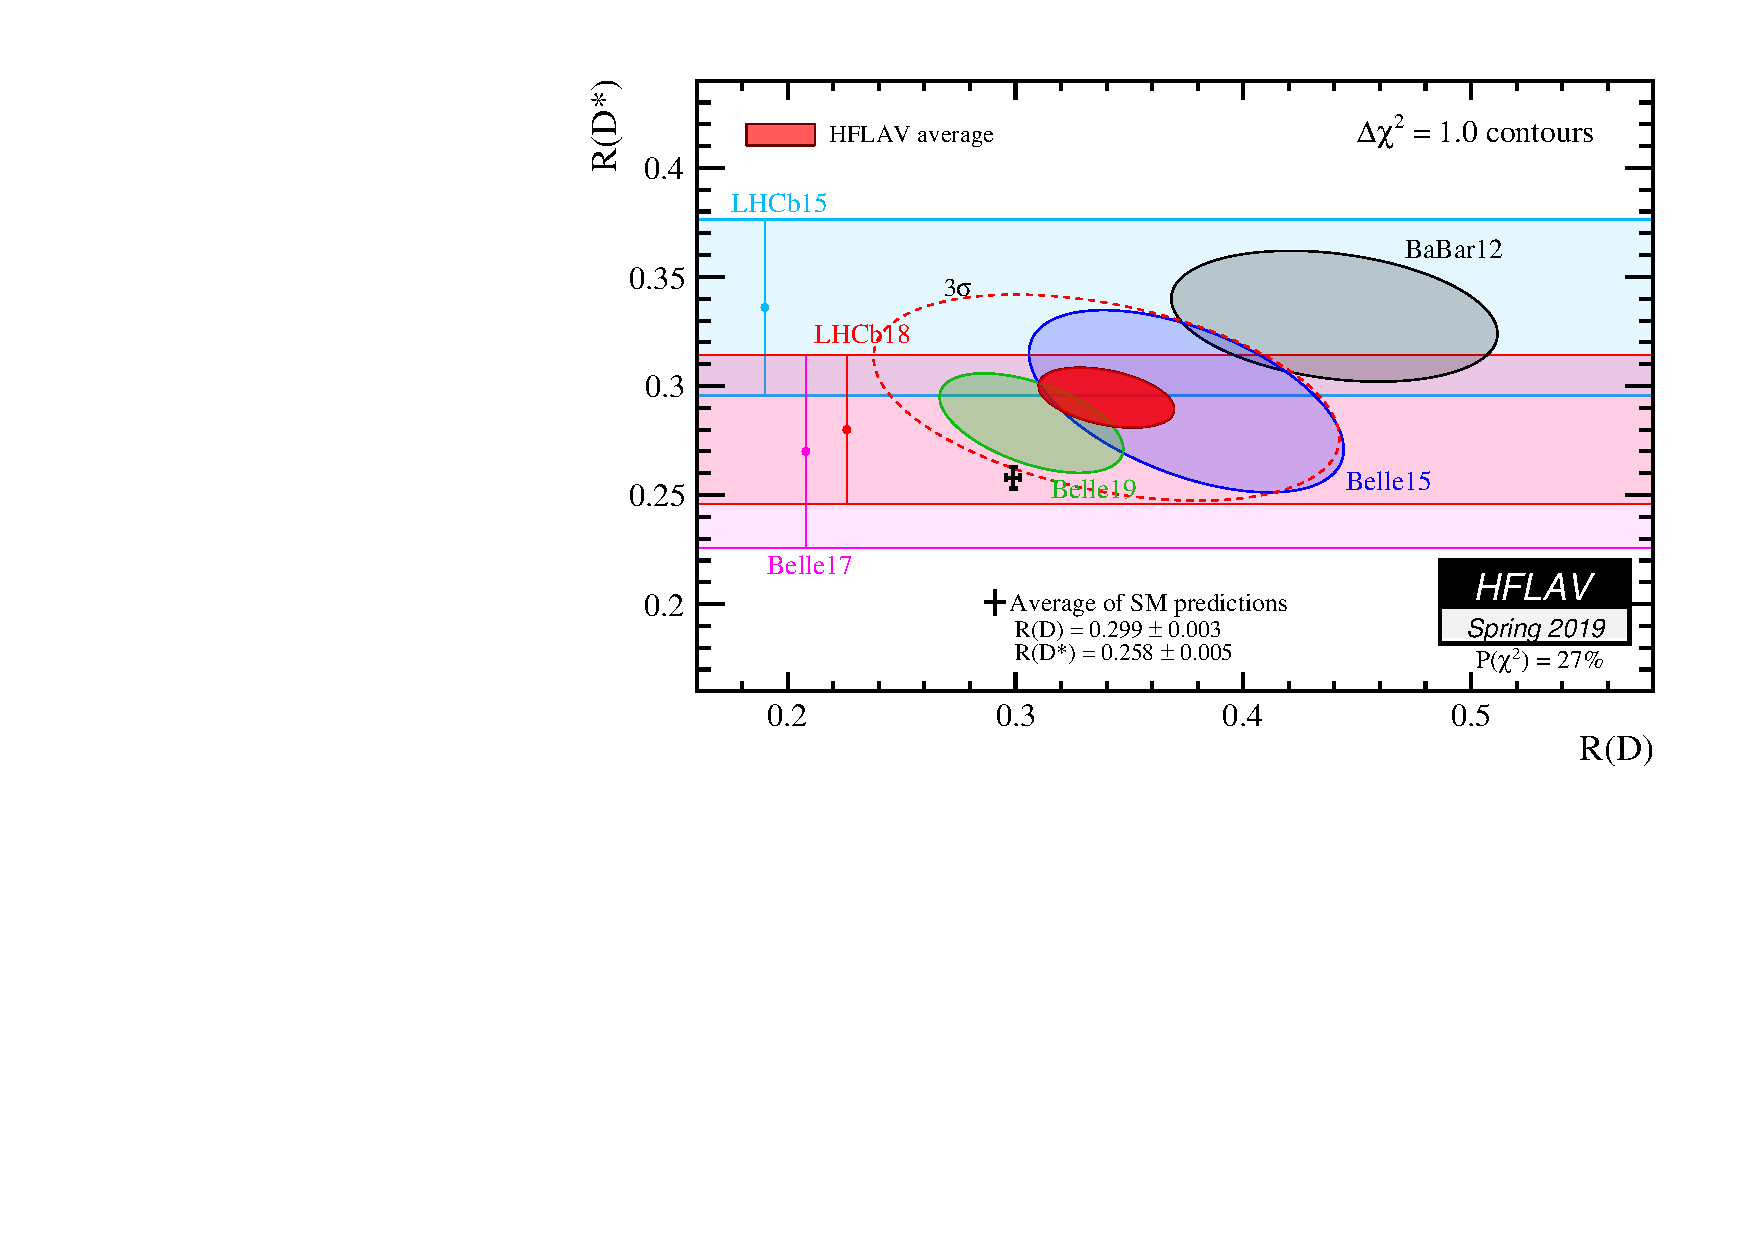
\includegraphics[width=\columnwidth]{figures/rdrds_spring2019.pdf}
        \end{column}
    \end{columns}
\footnotetext[2]{Y. S. Ahmis \textit{et al.} (HFLAV) arXiv:1909.12524}
\end{frame}

\begin{frame}\frametitle{Effective Field Theory}
    \setbeamercovered{transparent}
    \def\beamertemplatetransparentcoveredmedium{\setbeamercovered{transparent=50}}
    \beamertemplatetransparentcoveredmedium
    \begin{itemize}
        \item  EFT ``integrates out" heavy degrees of freedom above energy scale $\Lambda$, resulting in operators with dim $> 4$. The short-distance physics is encoded in the Wilson coefficient that multiplies each operator.
              $$\mathcal{L}_\mathrm{EFT} = \mathcal{L}_\mathrm{SM} + \frac{1}{\Lambda}\sum C^{(5)} \mathcal{O}^{(5)} + \frac{1}{\Lambda^2}\sum C^{(6)} \mathcal{O}^{(6)} + \cdots$$
              \vspace{-2mm}
        \item In particular, SMEFT integrates out all NP degrees of freedom.
              \begin{itemize}
                  \item Model-independent description.
                  \item 2499 dimension-6 operators ($\Delta B = \Delta L = 0$).
\item Warsaw basis\footnotemark[3] is the most common choice.
                  \item We will consider NP contributions to the following operators:
                        $$\mathcal{O}_{\ell q(1)}^{ijkl} = (\bar{\ell}_i \gamma_\mu \ell_j)(\bar{q}_k \gamma^\mu  q_l), \qquad \mathcal{O}_{\ell q(3)}^{ijkl} = (\bar{\ell}_i \gamma_\mu \tau^I \ell_j)(\bar{q}_k \gamma^\mu \tau^I q_l).$$
\footnotetext[3]{Grzadkowski, M. Iskrzynski, M. Misiak, J. Rosiek,    JHEP 10 (2010) 085. arXiv:1008.4884}
              \end{itemize}
    \end{itemize}
\end{frame}

\begin{frame}\frametitle{Effective Field Theory}
\begin{itemize}

\item The scale of $B$ decays is $\mu \approx m_b$. We need to integrate out $t$, $H$, $W$ and $Z$.

\item The Weak Effective Theory (WET) Lagrangian is given by
{\scriptsize $$\mathcal{L}_{\text{WET}} = \mathcal{L}_\mathrm{SM} -\frac{4 G_F}{\sqrt{2}}V_{cb}\sum_{\ell = e, \mu, \tau} (1 + C_{VL}^\ell) \mathcal{O}_{VL}^\ell + \frac{4G_F}{\sqrt{2}}V_{tb}V_{ts}^*\frac{e^2}{16\pi^2}\sum_{\ell=e,\mu} (C_9^\ell \mathcal{O}_9^\ell  + C_{10}^\ell \mathcal{O}_{10}^\ell) \ ,$$}
{ $$\mathcal{O}_{VL}^\ell = (\bar{c}_L \gamma_\alpha b_L)(\bar{\ell}_L \gamma^\alpha \nu_\ell)\ ,$$ $$\mathcal{O}_9^\ell = (\bar{s}_L \gamma_\alpha b_L)(\bar{\ell} \gamma^\alpha \ell)\ , \qquad \mathcal{O}_{10}^\ell = (\bar{s}_L \gamma_\alpha b_L)(\bar{\ell} \gamma^\alpha \gamma_5 \ell) \ .$$}

\item $\mathcal{O}_{VL}^\ell$ contributes to $R_{D^{(*)}}$ and $\mathcal{O}_9^\ell$, $\mathcal{O}_{10}^\ell$ to $R_{K^{(*)}}$

\item To relate the Wilson coefficients at both scales:
\begin{enumerate}
    \item Run the SMEFT RG equations from $\Lambda$ down to EW scale.
    \item Match the SMEFT operators to the WET operators.
    \item Run the WET RG equations from EW scale down to $m_b$.
\end{enumerate}
    
\end{itemize}
\end{frame}

\begin{frame}\frametitle{Fit to complex WCs: Approach}
    Common explanation for anomalies in $R_{K^{(*)}}$ and $\Delta M_s$.
    \begin{itemize}
        \item $1.8\sigma$ tension with the 2017 theoretical SM prediction for $B_s$ mixing,\\
              $\Delta M_S^\mathrm{SM} = 20.01 \pm 1.25\,\mathrm{ps}^{-1}$, \qquad$\Delta M_S^\mathrm{exp} = 17.757 \pm 0.021 \,\mathrm{ps}^{-1}$. \footnotemark[4]
        \item $\mathcal{L}_{\Delta M_S} = -\frac{4 G_f}{\sqrt{2}} (V_{tb} V_{ts}^*)^2 C_{bs, \mathrm{NP}}^{LL} \mathcal{O}_{bs}^{LL} + \mathrm{h. c.}$
              \begin{itemize}
                  \item $ \mathcal{O}_{bs}^{LL} = (\bar{s}_L \gamma_\mu b_L)^2$.
                  \item $\Delta M_S = \Delta M_S^\mathrm{SM} \left|1 + \frac{C_{bs}^{LL} }{R^\mathrm{loop}} \right|$.
                  \item CP asymmetry\footnotemark[4]: $\ACPmix (B_s\to J/\psi \phi)= \sin \left[\mathrm{arg}\left(   1 + \frac{C_{bs}^{LL} }{R^\mathrm{loop}} \right) - 2 \beta_s \right] $.
              \end{itemize}
    \end{itemize}

    ~

    We need a model-dependant connection between $R_{K^{(*)}}$ and $\Delta M_s$:
    \begin{itemize}
        \item $Z'$: $\mathcal{L}_{Z'} \sim \lambda^Q \bar{d}\gamma^\mu d Z'_\mu + \lambda^L \bar{e}\gamma^\mu e Z'_{\mu}$.
        \item Leptoquarks ($S_3$): $\mathcal{L}_{S_3} \sim y^{QL} \bar{q} \ell S_3$.
    \end{itemize}
    \footnotetext[4]{{L. Di Luzio, M. Kirk, A. Lenz. arXiv:1712.06572}}
\end{frame}

\begin{frame}\frametitle{Fit to complex WCs: $Z'$ model}
    \begin{itemize}
        \item $\mathcal{L}_{Z'} =  \frac{1}{2} M_{Z'}^2 (Z'_\mu)^2 + (\lambda_{ij}^Q \bar{d}^i_L \gamma^\mu d^j_L + \lambda_{\alpha\beta}^L \bar{e}^\alpha_L \gamma^\mu e_L^\beta )Z'_\mu $.~\\~\\
        \item $C_9^\mu = - C_{10}^\mu = \frac{-\pi}{\sqrt{2} G_F \alpha V_{tb} V_{ts}^*}\frac{\lambda^Q_{23}}{M_{Z'}^2}\qquad\qquad [\lambda^L_{22} = 1]$.
        \item $C_{bs}^{LL} = \frac{\eta^{LL}}{4\sqrt{2}G_F (V_{tb} V_{ts}^*)^2}\left(\frac{\lambda_{23}^Q}{M_{Z'}}\right)^2$. \footnote[4]{L. Di Luzio, M. Kirk, A. Lenz. arXiv:1712.06572}
    \end{itemize}

    \begin{columns}
        \begin{column}[t]{0.48\textwidth}
            \begin{figure}
                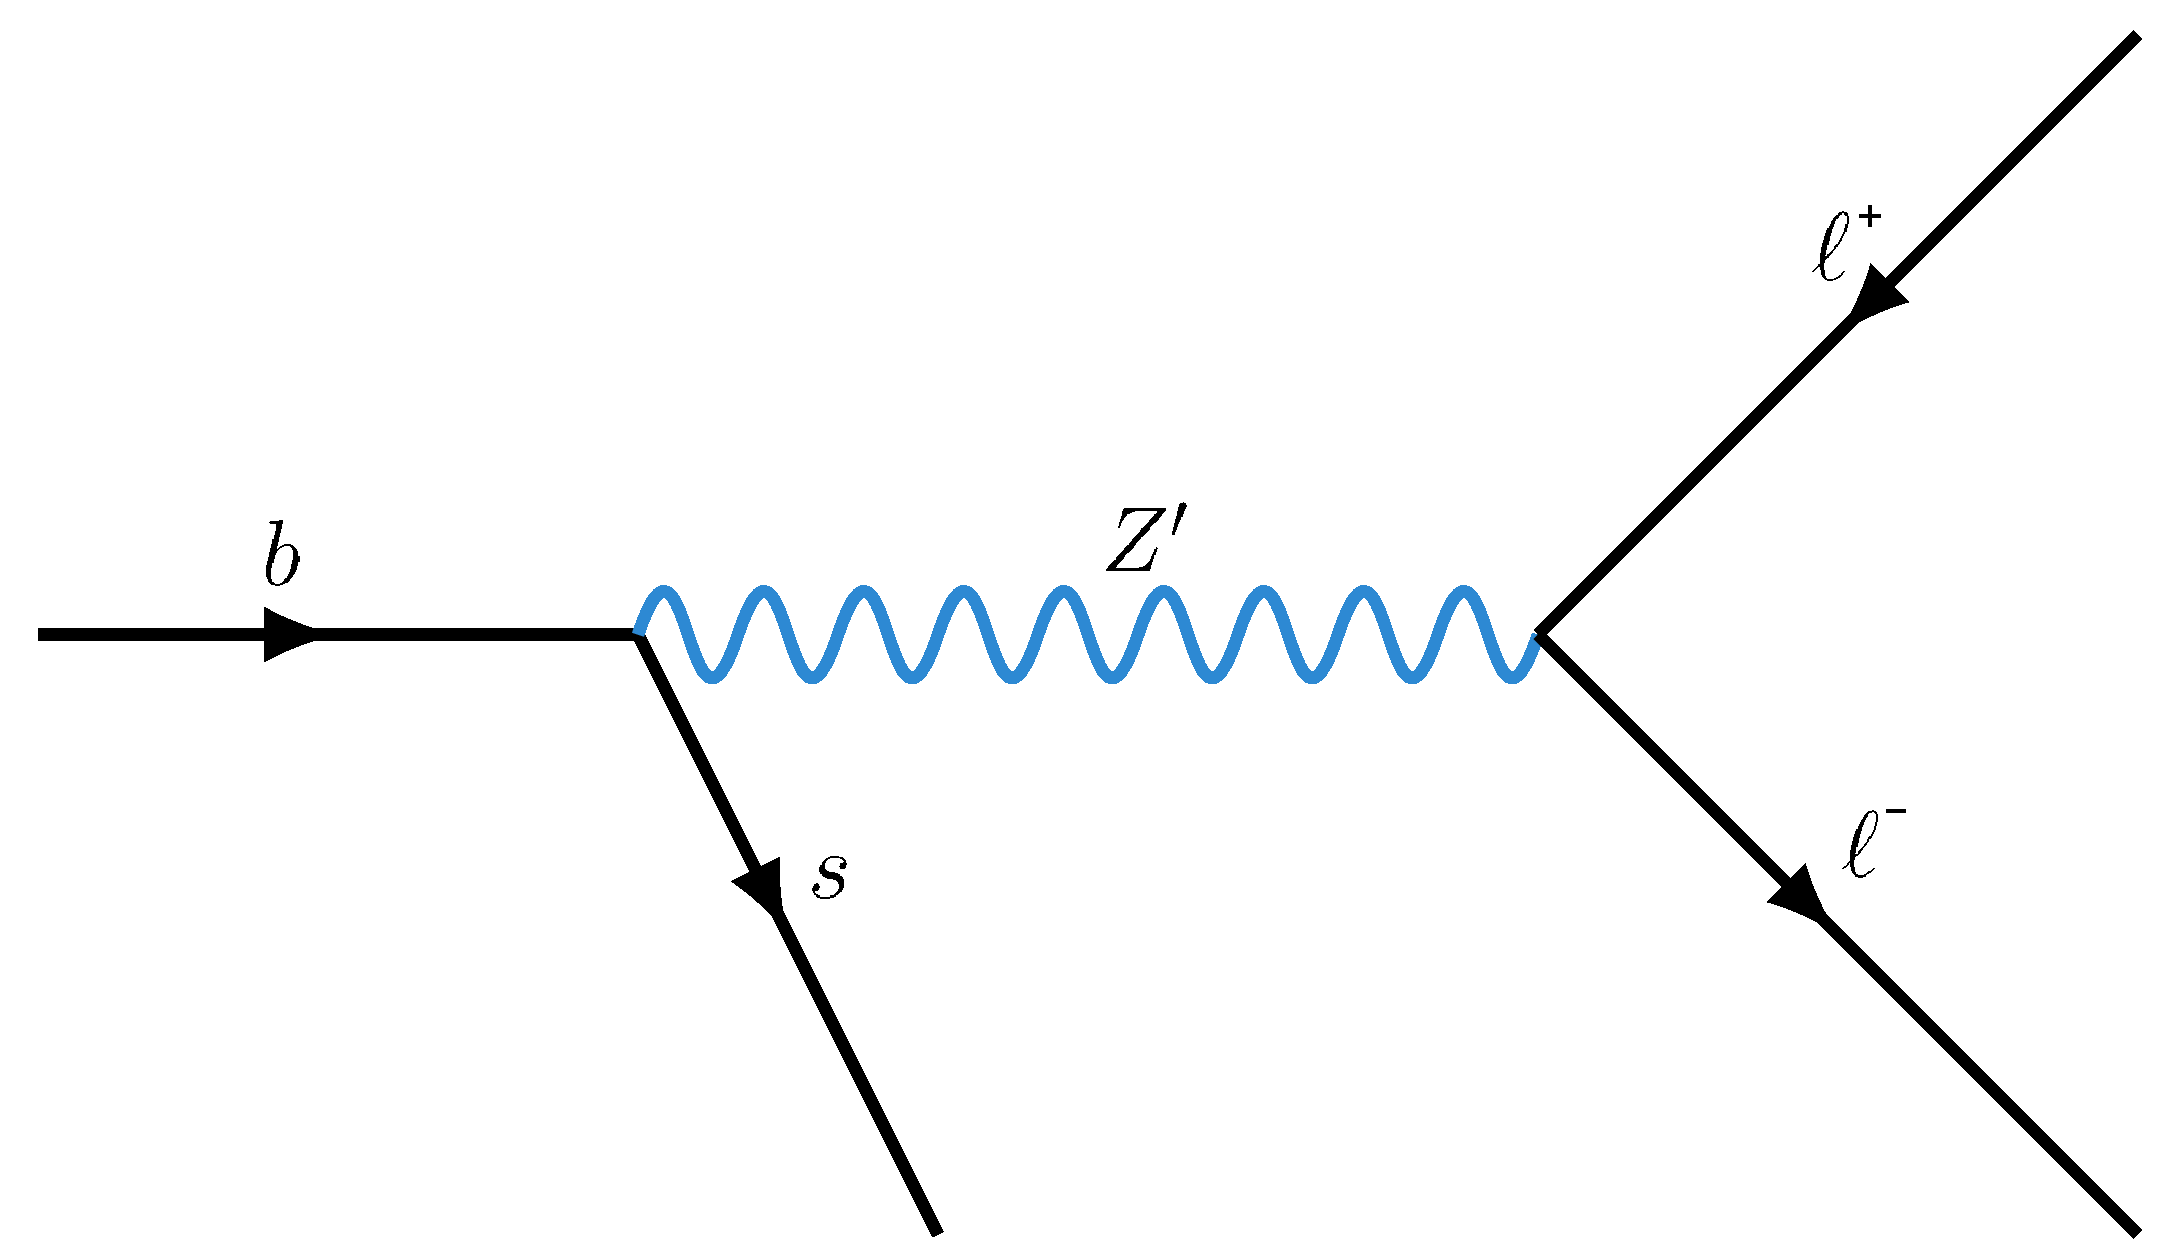
\includegraphics[width=0.7\textwidth]{figures/feynZLFUV.png}
            \end{figure}
        \end{column}
        \begin{column}[t]{0.48\textwidth}
            \begin{figure}
                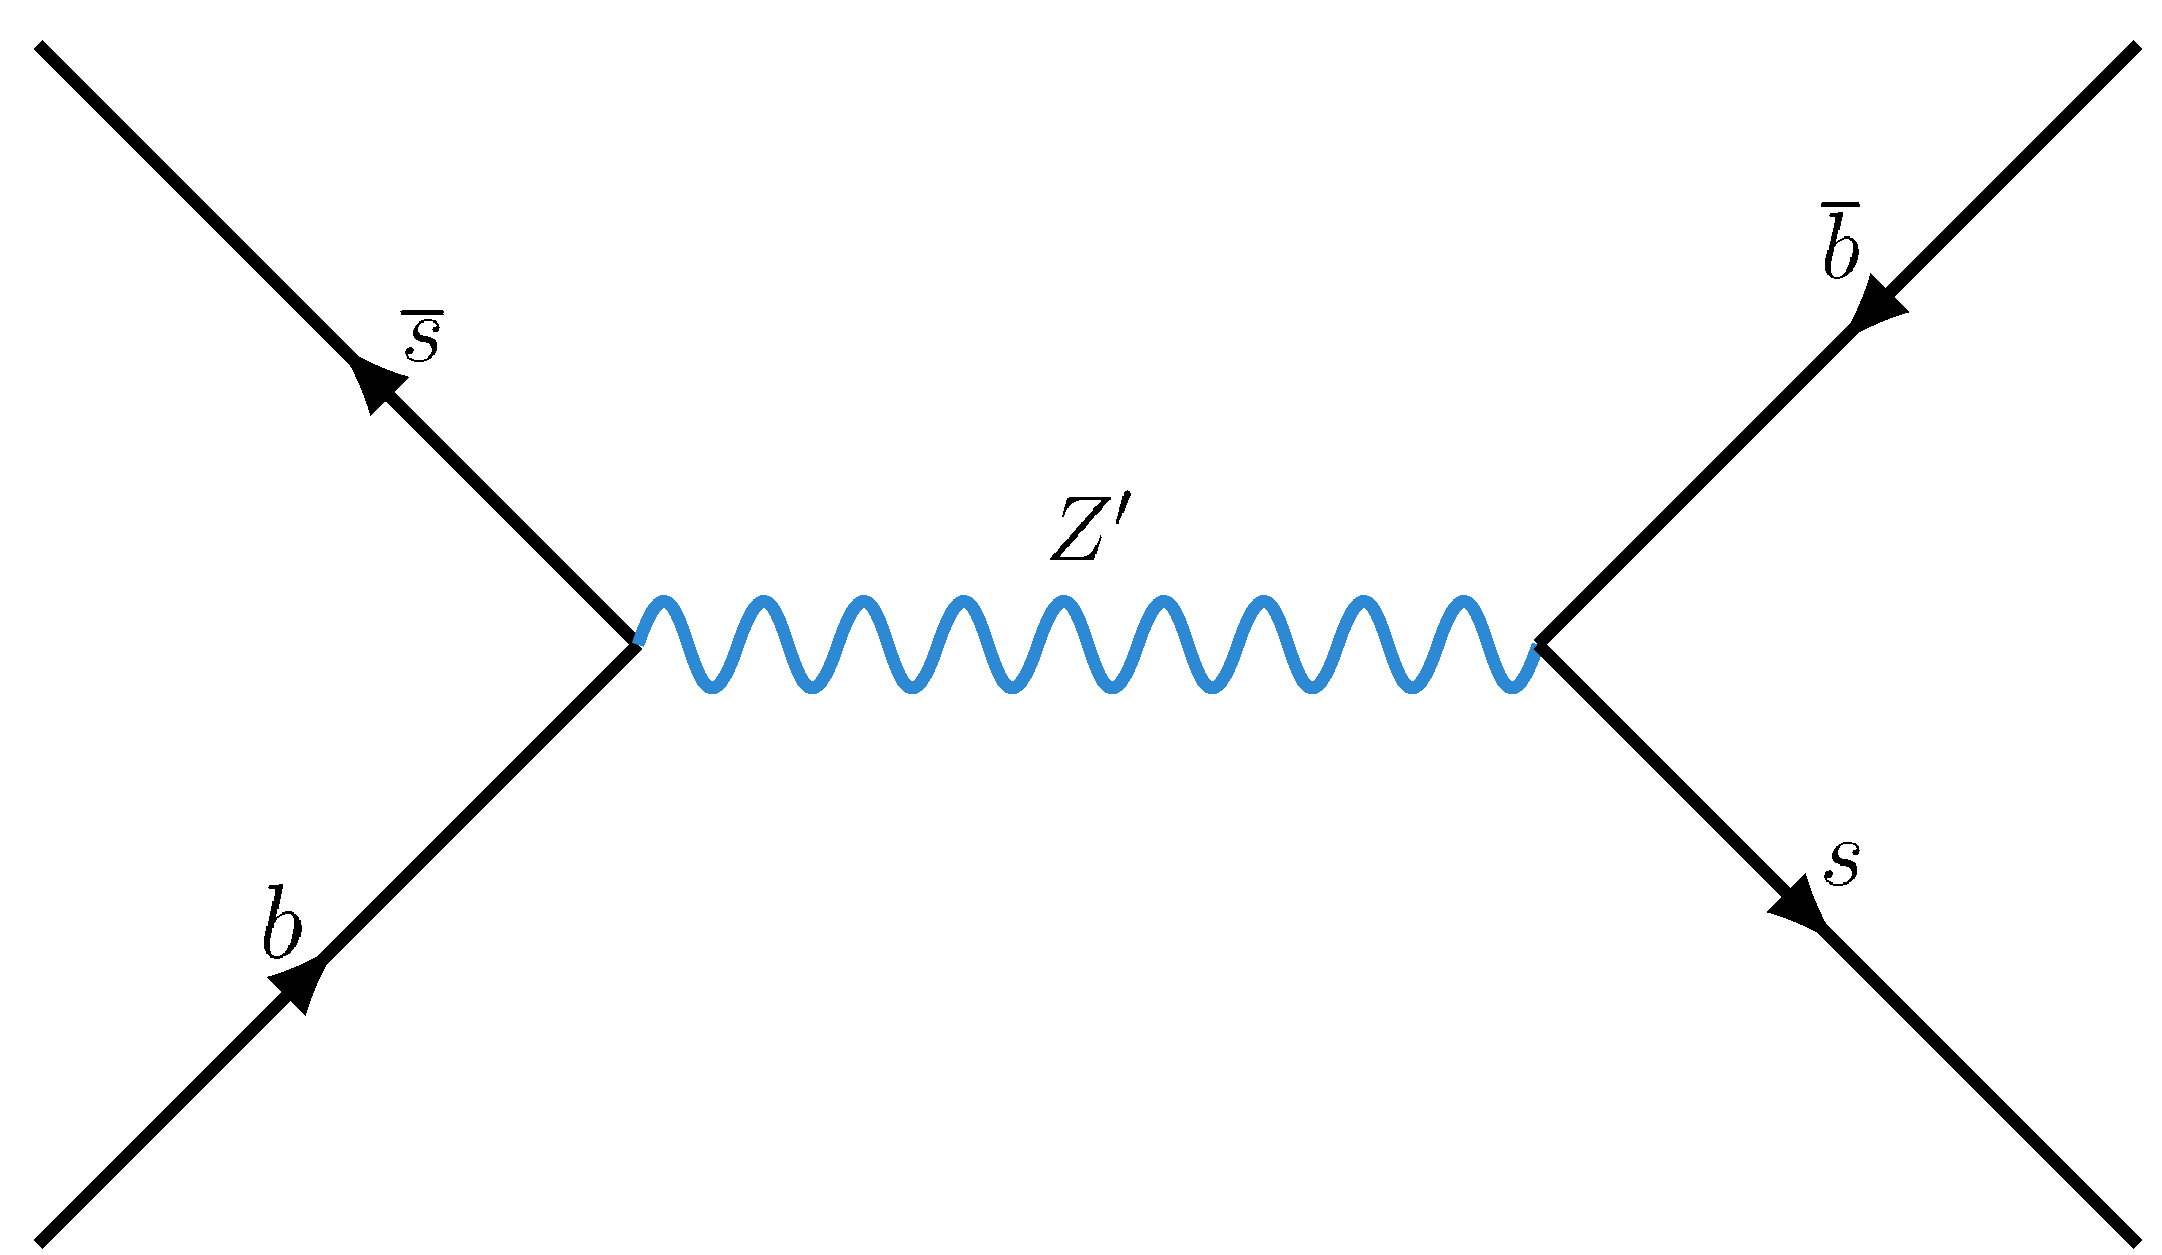
\includegraphics[width=0.7\textwidth]{figures/feynZBs.png}
            \end{figure}
        \end{column}
    \end{columns}
\end{frame}

\begin{frame}\frametitle{Fit to complex WCs: Leptoquark $S_3$ model}
    \begin{itemize}
        \item $\mathcal{L}_{S_3} = -M^2_{S_3} |S_3^a|^2 + y_{i\alpha}^{QL} \bar{q^c}^i (\epsilon \sigma^a) \ell^\alpha S_3^a  + \mathrm{h.c.}$~\\~\\
        \item $C_9^\mu = -C_{10}^\mu = \frac{\pi}{\sqrt{2} G_F \alpha V_{tb} V_{ts}^*} \frac{y^{QL}_{32} y^{QL*}_{22}}{M^2_{S_3}}$.
        \item $C_{bs}^{LL} = \frac{5\eta^{LL}}{256 \sqrt{2} \pi^2 G_F (V_{tb} V_{ts}^*)^2}\left(\frac{y^{QL}_{3\alpha} y^{QL*}_{2\alpha}}{M_{S_3}}\right)^2$. \footnote[4]{L. Di Luzio, M. Kirk, A. Lenz. arXiv:1712.06572}
    \end{itemize}

    \begin{columns}
        \begin{column}[t]{0.48\textwidth}
            \begin{figure}
                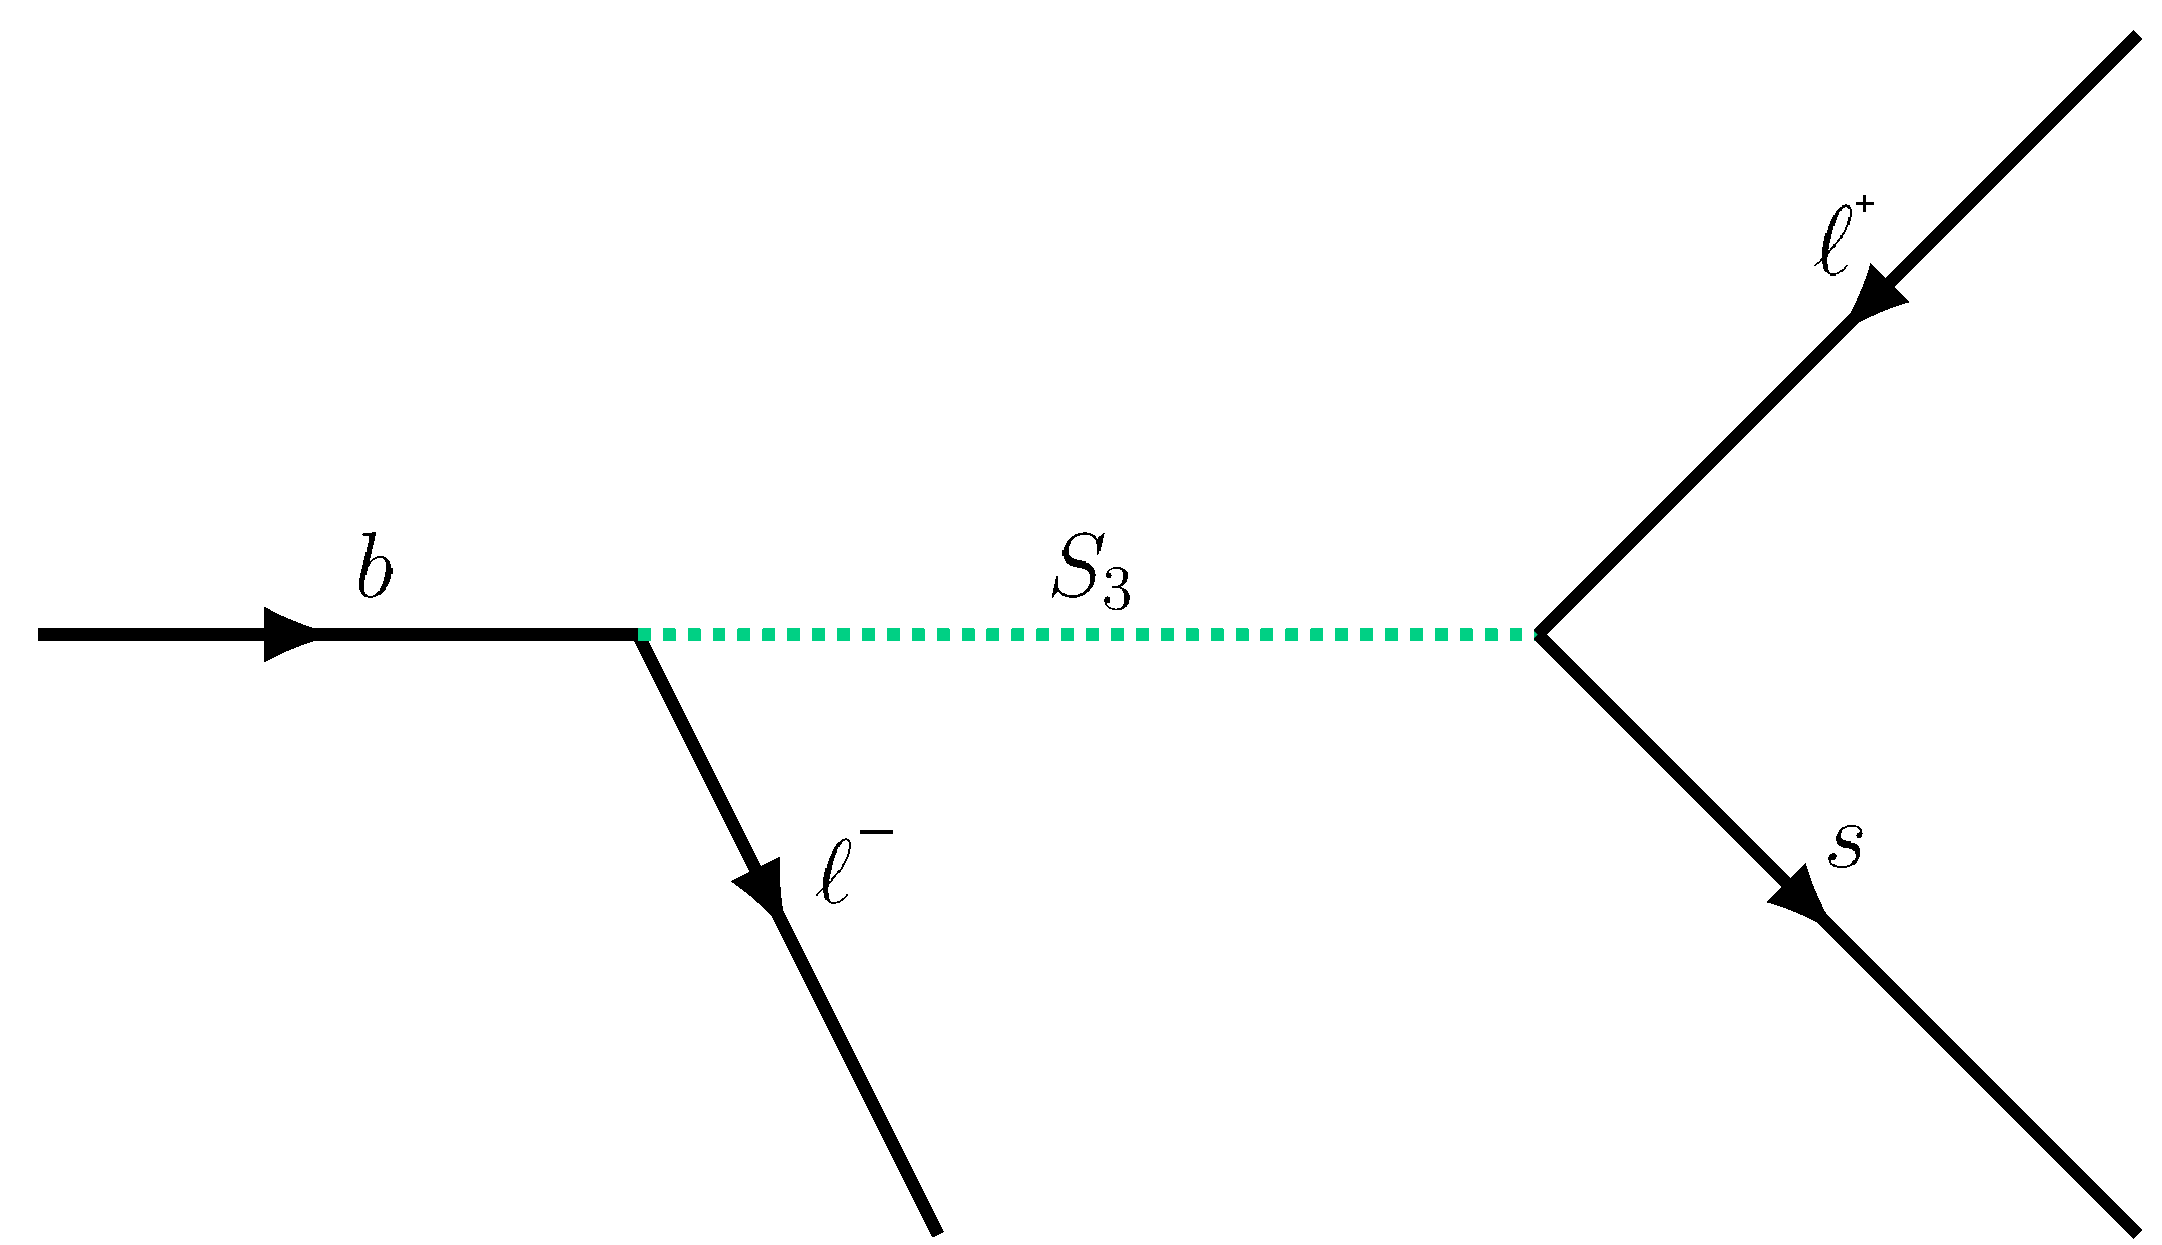
\includegraphics[width=0.7\textwidth]{figures/feynLQLFUV.png}
            \end{figure}
        \end{column}
        \begin{column}[t]{0.48\textwidth}
            \begin{figure}
                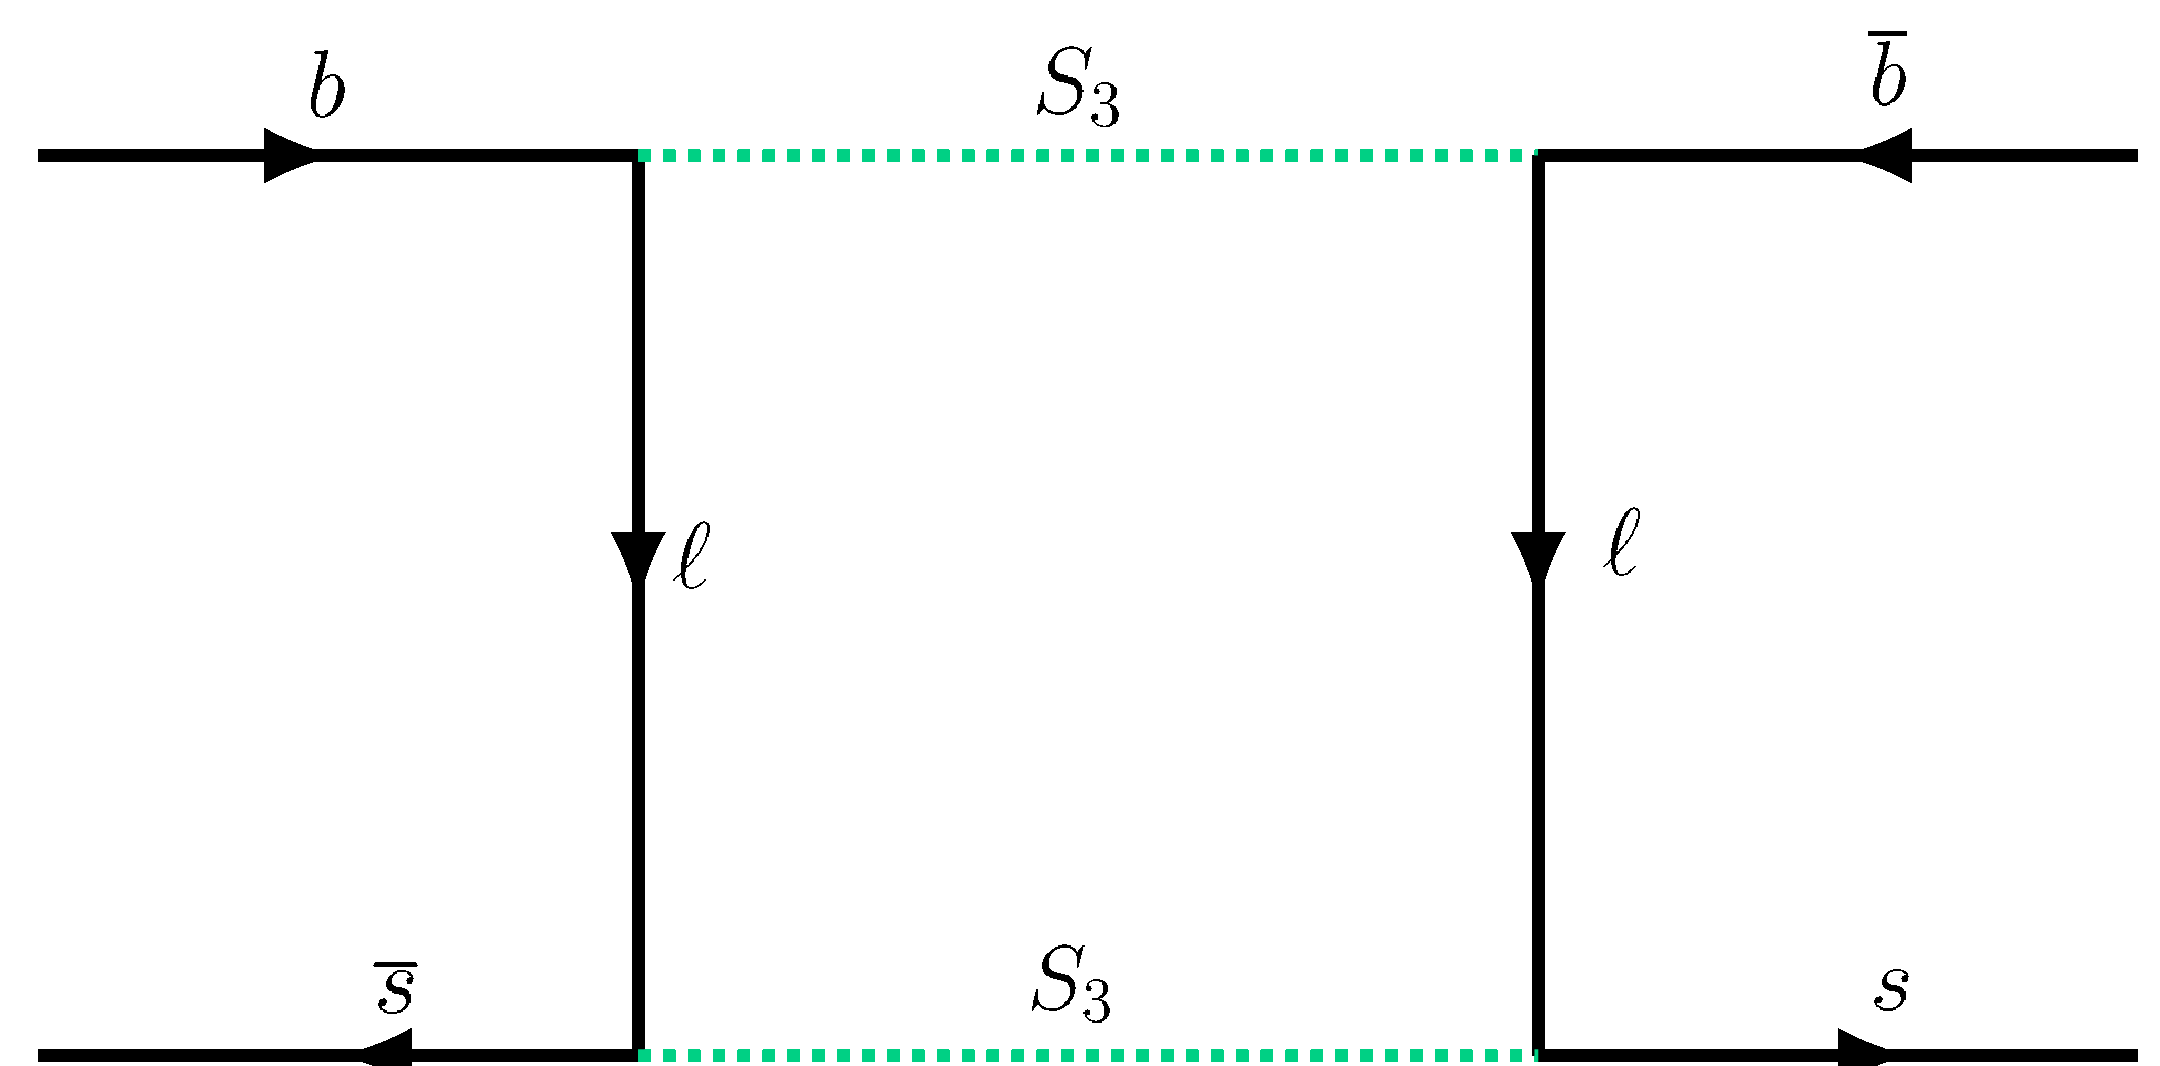
\includegraphics[width=0.7\textwidth]{figures/feynLQBs.png}
            \end{figure}
        \end{column}
    \end{columns}
\end{frame}

\begin{frame}\frametitle{Fit to complex WCs: Real case}
    \begin{columns}
        \begin{column}[t]{0.48\textwidth}
            \begin{figure}
                \centering
                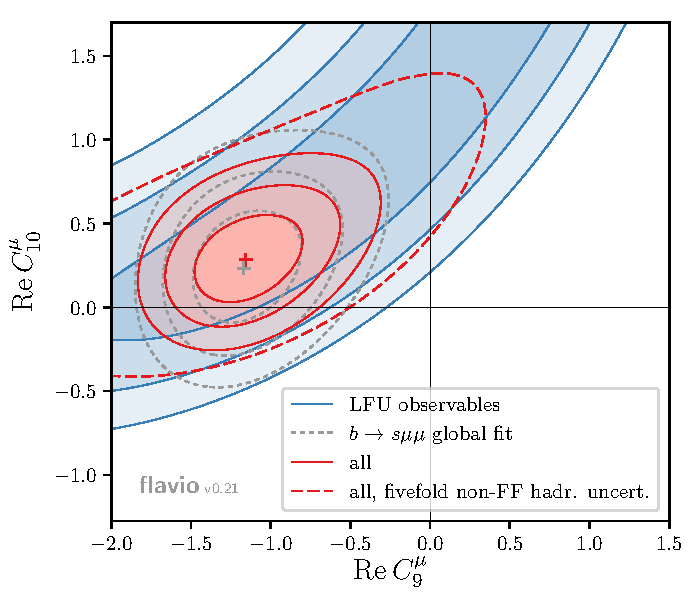
\includegraphics[width =0.9\textwidth]{figures/contours_cropped.pdf}\\
                \small{Allowed real $C_9$ and $C_{10}$ \\coefficients. \protect\footnotemark[7]}
            \end{figure}
        \end{column}\footnotetext[7]{W. Altmannshofer, P. Stangl, D. M. Straub.  arXiv:1704.05435}
        \begin{column}[t]{0.48\textwidth}
            \begin{figure}
                \centering
                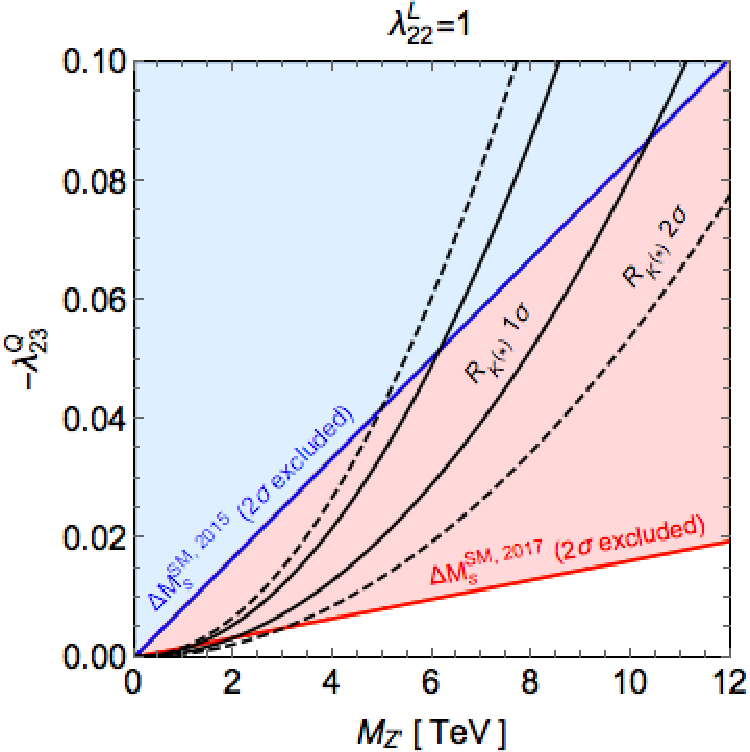
\includegraphics[width =0.8\textwidth]{figures/BsmixvsRK.pdf}\\
                \small{Bounds on $Z'$ couplings from $B_s$ mixing and $R_{K^{(*)}}$. \protect\footnotemark[8] }
            \end{figure}
        \end{column}\footnotetext[8]{L. Di Luzio, M. Kirk, A. Lenz. arXiv:1712.06572}
    \end{columns}
    \begin{itemize}
        \item \textbf{Problem:} Real values for the LQ/$Z'$ couplings increase $\Delta M_S^\mathrm{NP}$.
        \item Why not \alert{imaginary or complex} couplings?
    \end{itemize}
\end{frame}

\begin{frame}\frametitle{Fit to complex WCs: $C_9$ and $C_{10}$}
    \begin{columns}
        \begin{column}[t]{0.48\textwidth}
            \begin{figure}
                \centering
                \includegraphics[width=0.95\textwidth]{figures/fitim_C9C10.pdf}\\
                Allowed imaginary Wilson coefficients.
            \end{figure}
        \end{column}
        \begin{column}[t]{0.48\textwidth}
            \begin{figure}
                \centering
                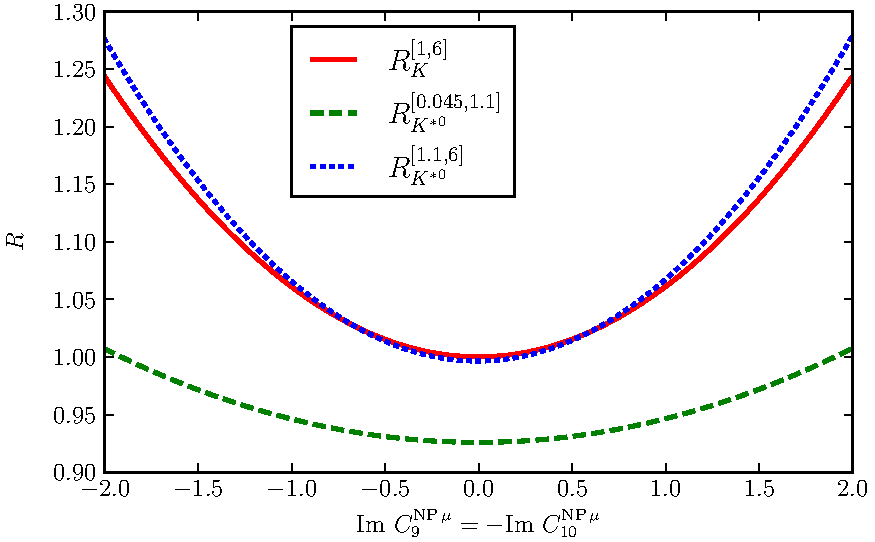
\includegraphics[width=0.95\textwidth]{figures/RK_im.pdf}\\
                Values of $R_{K^{(*)}}$ with imaginary Wilson coefficients.
            \end{figure}
        \end{column}
    \end{columns}

    ~

    \begin{table}
        \centering
        \begin{tabular}{|l|c|c|}\hline
            \textbf{Best fits} & $C_9^\mu=-C_{10}^\mu$ & $\sqrt{\chi^2_\mathrm{SM} - \chi^2_\mathrm{fit}}$ \\\hline
            Real               & $ -0.86$              & $6.0 $                                            \\\hline
            Imaginary          & $-0.005\;i $          & $0.02 $                                           \\\hline
            Complex            & $-1.16\pm 1.14\;i$    & $6.1$                                             \\\hline
        \end{tabular}
    \end{table}
\end{frame}

\begin{frame}\frametitle{Fit to complex WCs: Fit to $Z'$ couplings}
    Fit to $R_K$, $R_{K^*}$, $P_4'$, $P_5'$, $\mathcal{B}(B_s \to \mu^+ \mu^-)$, $\Delta M_S$, $A_\mathrm{CP}^\mathrm{mix}(B_s \to J/\psi\, \phi)$.

    \begin{figure}
        \begin{columns}
            \begin{column}{0.48\textwidth}
                \centering
                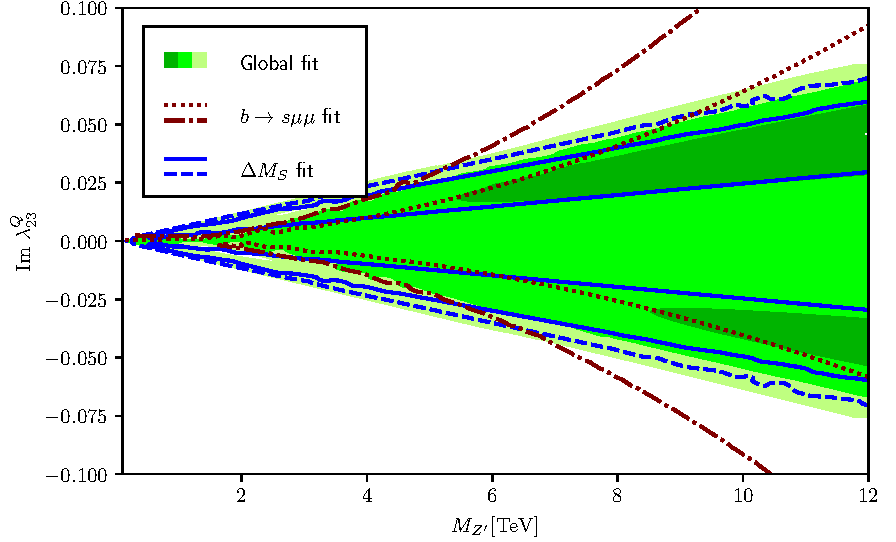
\includegraphics[width=0.9\textwidth]{figures/fitim_Z.pdf}
                \\ {\small Imaginary $Z'$ fit.}
            \end{column}
            \begin{column}{0.48\textwidth}
                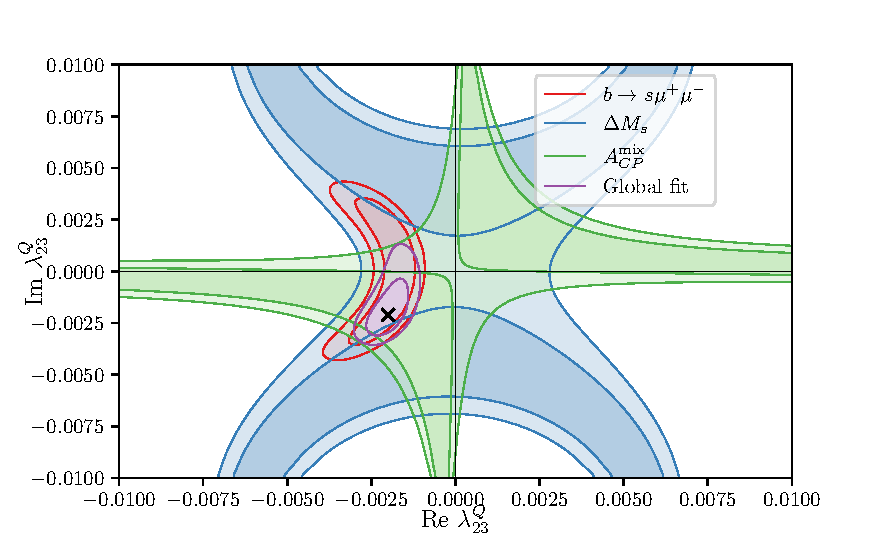
\includegraphics[width=0.9\textwidth]{figures/fitcompl_Z.pdf}
                \\ {\small Complex $Z'$ fit.}

            \end{column}
        \end{columns}
    \end{figure}
    \begin{table}
        \centering
        \begin{tabular}{|l|c|c|c|}\hline
            \textbf{Best fits} & $\lambda^Q_{23}$    & $M_{Z'}$             & $\sqrt{\chi^2_\mathrm{SM} - \chi^2_\mathrm{fit}}$ \\\hline
            Real               & $-0.002$            & $1.31\,\mathrm{TeV}$ & $5.70$ \quad (\alert{$5.39\sigma$})               \\\hline
            Imaginary          & $\pm 0.047\;i$      & $12\,\mathrm{TeV}$   & $1.61$  \quad (\alert{$1.1\sigma$})               \\\hline
            Complex            & $-0.0020-0.0021\;i$ & $1.08\,\mathrm{TeV}$ & $6.05$ \quad (\alert{$5.43\sigma$})               \\\hline
        \end{tabular}
    \end{table}

    The better fit is provided by complex couplings.
\end{frame}

\begin{frame}\frametitle{Fit to complex WCs: Fit to $S_3$ couplings}
    Fit to $R_K$, $R_{K^*}$, $P_4'$, $P_5'$, $\mathcal{B}(B_s \to \mu^+ \mu^-)$, $\Delta M_S$, $A_\mathrm{CP}^\mathrm{mix}(B_s \to J/\psi\, \phi)$.

    \begin{figure}
        \begin{columns}
            \begin{column}{0.48\textwidth}
                \centering
                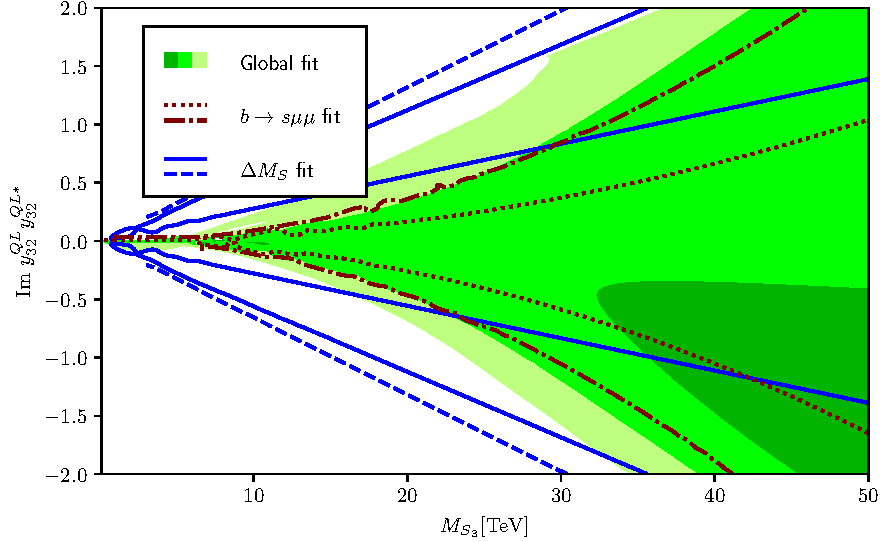
\includegraphics[width=0.9\textwidth]{figures/fitim_LQ.pdf}
                \\ {\small Imaginary $S_3$ fit.}
            \end{column}
            \begin{column}{0.48\textwidth}
                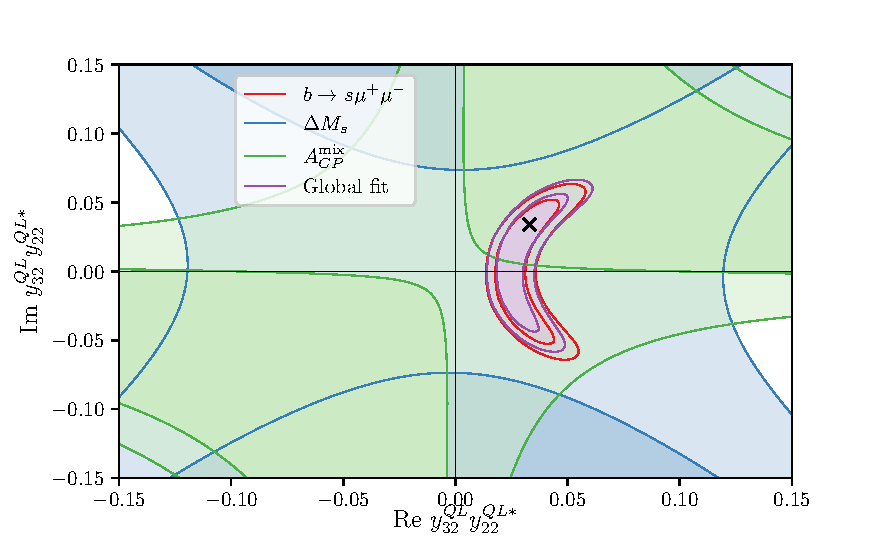
\includegraphics[width=0.9\textwidth]{figures/fitcompl_LQ.pdf}
                \\ {\small Complex $S_3$ fit.}

            \end{column}
        \end{columns}
    \end{figure}

    \begin{table}
        \centering
        \begin{tabular}{|l|c|c|c|}\hline
            \textbf{Best fits} & $y^{QL}_{32} y^{QL*}_{22}$ & $M_{S_3}$            & $\sqrt{\chi^2_\mathrm{SM} - \chi^2_\mathrm{fit}}$ \\\hline
            Real               & $ 0.04 $                   & $5.19\,\mathrm{TeV}$ & $5.82$ \quad (\alert{$5.47\sigma$})               \\\hline
            Imaginary          & $-1.67\;i$                 & $50\,\mathrm{TeV}$   & $1.15$ \quad (\alert{$0.6\sigma$})                \\\hline
            Complex            & $0.033+0.034\;i$           & $4.10\,\mathrm{TeV}$ & $5.90$ \quad (\alert{$5.27\sigma$})               \\\hline
        \end{tabular}
    \end{table}

\end{frame}

\begin{frame}\frametitle{Fit to complex WCs: Observables}

    \begin{figure}
        \begin{columns}
            \begin{column}{0.48\textwidth}
                \centering
                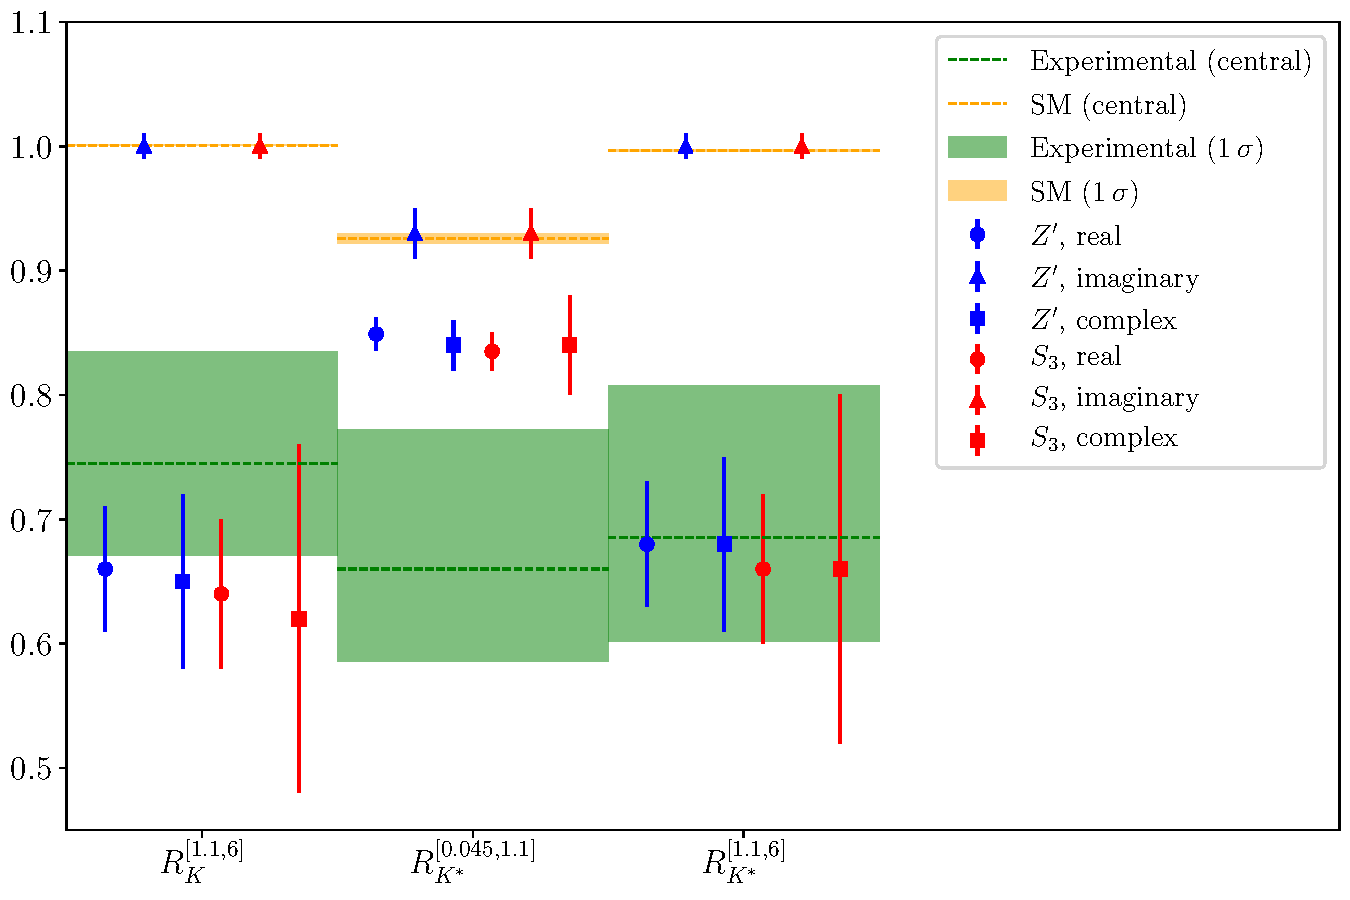
\includegraphics[width = 0.8\textwidth]{figures/errorplot_RKmodels.pdf}
            \end{column}
            \begin{column}{0.48\textwidth}
                $1\sigma$ intervals for observables in the {\color{blue}$Z'$} and {\color{red} LQ} fits, compared to the {\color{green} experimental values} and {\color{orange} SM predictions}.


            \end{column}
        \end{columns}
    \end{figure}
    \begin{figure}
        \begin{columns}
            \begin{column}{0.48\textwidth}
                \centering
                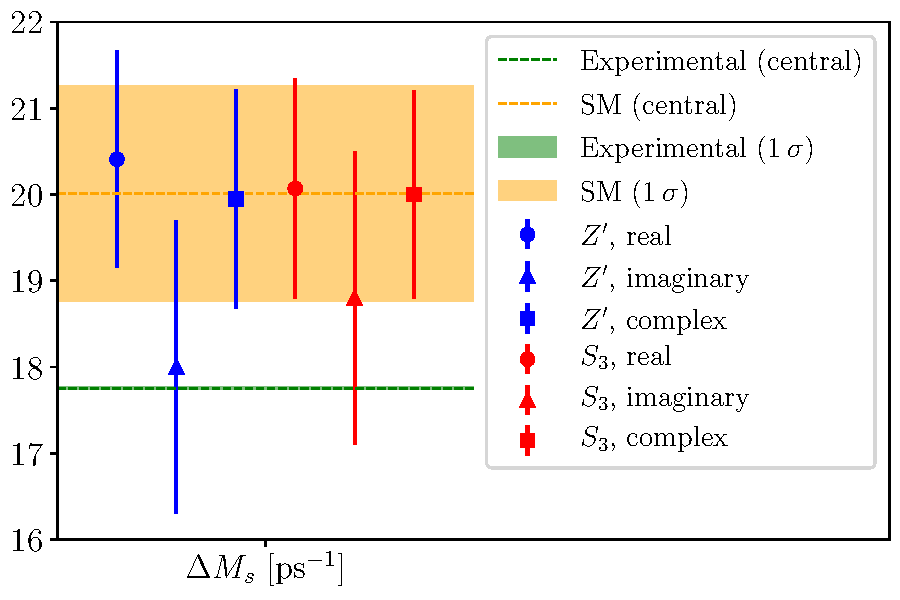
\includegraphics[width = 0.8\textwidth]{figures/errorplot_DMsmodels.pdf}
            \end{column}
            \begin{column}{0.48\textwidth}
                \centering
                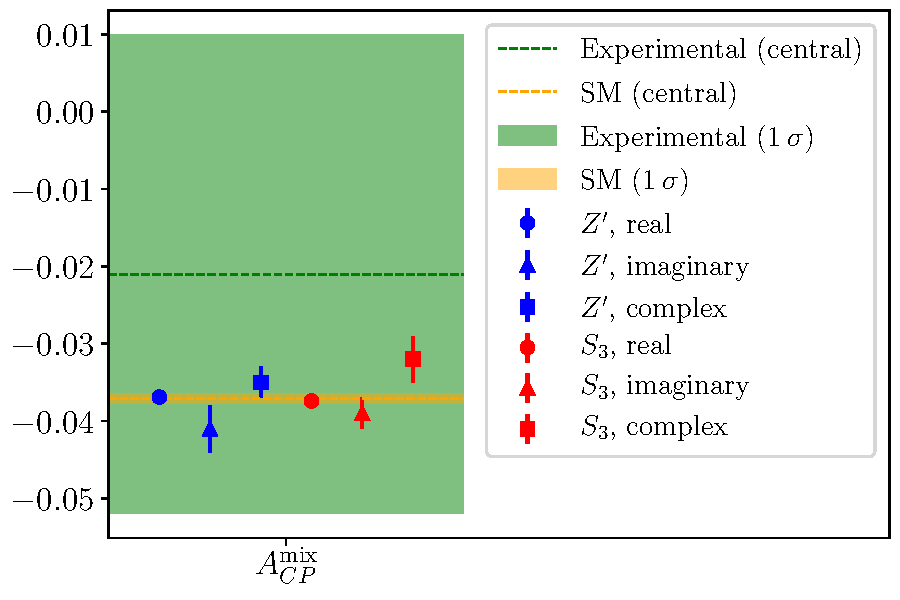
\includegraphics[width = 0.8\textwidth]{figures/errorplot_ACPmodels.pdf}
            \end{column}
        \end{columns}
    \end{figure}
\end{frame}

\begin{frame}\frametitle{Fit to complex WCs: Conclusions}
    \begin{itemize}
        \item Hints of New Physics violating Lepton Flavour Universality in the $B$ sector.
        \item Characterization using EFT and model building.
        \item Real Wilson coefficients cannot explain the $B_S$ mixing anomaly; imaginary Wilson coefficients cannot explain the $R_{K^{(*)}}$ anomaly.
        \item Complex couplings offer a slightly better global fit.

    \end{itemize}

\end{frame}

\begin{frame}\frametitle{Fit to complex WCs: Update}
    \begin{itemize}
        \item The SM prediction for $\Delta M_S$ was updated in 2019 to $\Delta M_S = (18.4^{+0.7}_{-1.2}) \mathrm{ps}^{-1}$,\footnote[9]{L. Di Luzio, M. Kirk, A. Lenz, and T. Rauh, arXiv:1909.11087} compatible with experiment.
        \item Therefore, imaginary or complex WC are no longer necessary. In the following fits we only consider real parameters.
        \item After the 2019 and 2021 $R_K$ measurements by LHCb, our results are not compatible with experimental data.
    \end{itemize}

    \begin{center}
        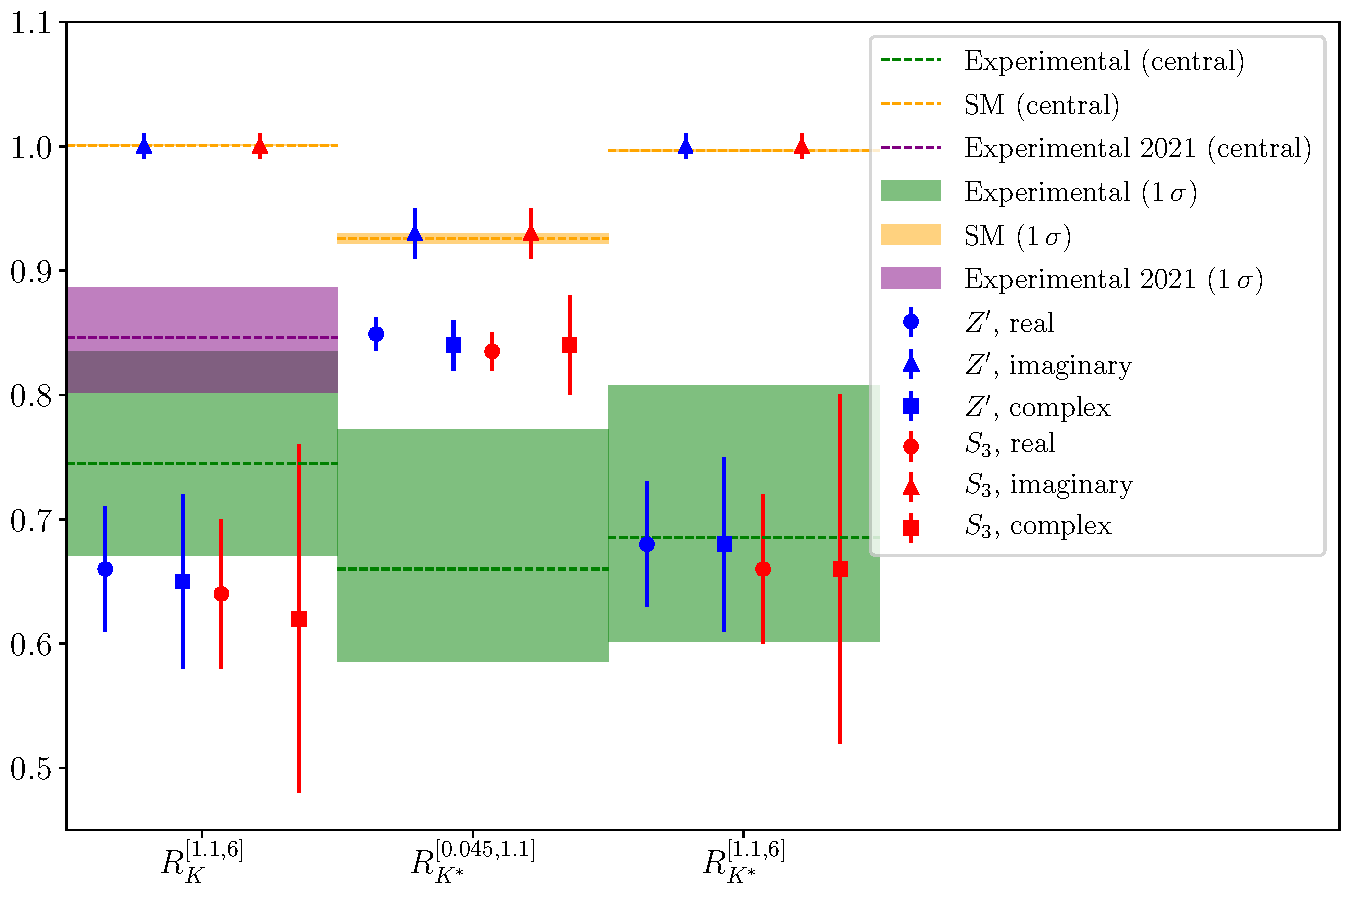
\includegraphics[width=0.6\textwidth]{figures/errorplot_RK2021.pdf}
    \end{center}

\end{frame}

\end{document}